\chapter{Introdução ao React com Expo e Docker}

\section{O que é o React?}



O React é uma biblioteca JavaScript para construção de interfaces de usuário. Criado por Jordan Walke no Facebook em 2011, foi tornado open-source em 2013. Desde então, tornou-se amplamente utilizado tanto no desenvolvimento web quanto no mobile, principalmente com o surgimento do React Native.


\section{Por que usar React?}

Entre os principais motivos para utilizar o React estão:

\begin{itemize}
  \item Componentização: permite criar interfaces como blocos reutilizáveis.
  \item Virtual DOM: atualizações eficientes sem recarregar toda a página.
  \item Grande comunidade e ecossistema.
  \item Compatibilidade com frameworks e bibliotecas modernas.
  \item Suporte a múltiplas plataformas com React Native.
\end{itemize}

\section{Tutorial: Criando uma nova Aplicação React com Expo}

Neste tutorial, criaremos um projeto React com o framework Expo, utilizando Docker para isolar o ambiente de desenvolvimento. O Expo é uma ferramenta que facilita o desenvolvimento de aplicativos React Native e também oferece suporte para execução no navegador via `expo start --web` \cite{reactCreatingApp,expoTutorial}.

\subsection{Templates do Expo}

Ao criar um projeto com o Expo usando o comando `expo init`, o usuário pode escolher diferentes templates, conforme descrito na documentação oficial \cite{expoCreateExpo}.

\begin{longtable}{|p{3.5cm}|p{3.5cm}|p{6.5cm}|}
\hline
\textbf{Template} & \textbf{Descrição} & \textbf{Inclui} \\
\hline
blank & Projeto mínimo com JavaScript & React Native sem nenhuma biblioteca adicional \\
\hline
blank (TypeScript) & Igual ao blank, mas com TypeScript & TypeScript + suporte a tipos \\
\hline
tabs (JavaScript) & Projeto com navegação por abas & Navegação, organização de pastas, componentes prontos \\
\hline
tabs (TypeScript) & Mesmo que tabs, com TypeScript & Tabs + TypeScript + organização estruturada \\
\hline
\end{longtable}

Neste projeto, escolhemos o template `blank`.

\subsection{Criação do projeto com Docker}

Utilizamos Docker para criar o projeto React com Expo, garantindo um ambiente consistente entre diferentes sistemas operacionais.

\subsubsection*{Makefile}

\begin{lstlisting}[caption={Comando Make para criar o projeto com Expo}]
IMAGE_NAME=react-app
APP_DIR=app

init:
	mkdir -p $(APP_DIR)
	docker run --rm -it -v "$$(pwd)/$(APP_DIR)":/app -w /app node:18-alpine \
		sh -c "npm install -g expo-cli && \
		       expo init . --template blank --npm --yes && \
		       npx expo install react-dom react-native-web @expo/metro-runtime"

build:
	docker build -t $(IMAGE_NAME) .

start:
	docker run -it --rm -p 8081:8081 -v "$$(pwd)/$(APP_DIR)":/app $(IMAGE_NAME)
\end{lstlisting}

\subsubsection*{Explicação dos comandos Docker}

\begin{itemize}
  \item \texttt{--rm}: remove o container após o uso.
  \item \texttt{-it}: roda o container interativamente.
  \item \texttt{-v "$(pwd)/app":/app}: monta a pasta local `app` no diretório `/app` do container.
  \item \texttt{-w /app}: define o diretório de trabalho no container.
\end{itemize}

\subsubsection*{Dockerfile}

\begin{lstlisting}[caption={Dockerfile}]
FROM node:18-alpine

WORKDIR /app

COPY app/package*.json ./
RUN npm install

COPY app .

EXPOSE 8081

CMD ["npx", "expo", "start", "--web"]
\end{lstlisting}
Fonte: \cite{dockerReact}
\subsection{Rodando a aplicação}

Após a criação e build da imagem, executamos:

\begin{lstlisting}[language=bash]
make init    # Executa uma vez para criar o projeto
make build   # Constrói a imagem Docker
make start   # Inicia o app em http://localhost:8081
\end{lstlisting}

\section{Desenvolvimento no navegador com Snack}

O Expo também oferece uma plataforma chamada \textbf{Snack}, que permite criar, editar e testar aplicações React Native diretamente no navegador, de forma semelhante ao CodePen ou CodeSandbox.

\begin{quote}
Essa solução é oferecida pelo próprio Expo e se chama Snack. O Snack é a solução de desenvolvimento React Native web do Expo. Com ele, conseguimos criar projetos completos e emular seu funcionamento diretamente no navegador. Algo muito parecido com o que temos com outras ferramentas web, tais como: CodePen (https://codepen.io/) e CodeSandBox (https://codesandbox.io/).
\end{quote}

\begin{quote}
Esta solução pode ser acessada diretamente pelo site oficial (https://snack.expo.dev/). O editor é bastante poderoso e oferece recursos avançados. É possível escolher a versão do Expo, conectar os apps com o seu dispositivo (de forma semelhante a que fizemos anteriormente), configurar atalhos e até mesmo mudar o tema para claro ou escuro.
\end{quote}

\section{Arquivos gerados pelo Expo}

Após a criação do projeto, os principais arquivos e pastas gerados são:

\begin{itemize}
  \item \texttt{package.json}: gerencia dependências e scripts.
  \item \texttt{index.js}: é o ponto de entrada principal de uma aplicação React.
  \item \texttt{App.js}: componente principal da aplicação.
  \item \texttt{assets/}: todos os arquivos estáticos da nossa aplicação, como, por exemplo, as imagens. Todas as imagens que vamos utilizar em nosso app deverão ser colocadas nessa pasta. 
  \item \texttt{/node\_modules}, onde estão contidas as dependências do projeto.
\end{itemize}


\subsection*{index.js}
\begin{lstlisting}[language=JavaScript, caption={Conteúdo de index.js}]
import { registerRootComponent } from 'expo';

import App from './App';

// registerRootComponent calls AppRegistry.registerComponent('main', () => App);
// It also ensures that whether you load the app in Expo Go or in a native build,
// the environment is set up appropriately
registerRootComponent(App);

\end{lstlisting}

\subsection*{App.js}


\begin{lstlisting}[language=JavaScript, caption={Novo conteúdo de App.js}]
import React from 'react';
import { View, Text, StyleSheet } from 'react-native';

export default function App() {
  return (
    <View style={styles.container}>
      <Text style={styles.text}>Bem-vindo ao React com Expo!</Text>
    </View>
  );
}

const styles = StyleSheet.create({
  container: {
    flex: 1,
    justifyContent: 'center',
    alignItems: 'center'
  },
  text: {
    fontSize: 20,
    fontWeight: 'bold'
  }
});
\end{lstlisting}

No início do arquivo \texttt{App.js}, encontramos algumas importações essenciais para o funcionamento do React Native. Primeiramente, é importado o \texttt{React} da biblioteca principal, o que permite a utilização de seus recursos de componentização. Em seguida, são importados três elementos da biblioteca \texttt{react-native}: \texttt{StyleSheet}, \texttt{Text} e \texttt{View}. Esses componentes são convertidos em elementos nativos quando a aplicação é executada em diferentes plataformas (Android, iOS ou web). Também é importado o componente \texttt{StatusBar}, disponibilizado pelo Expo, que ajuda no controle visual da barra de status do dispositivo.

Na sequência, é declarada e exportada a função \texttt{App}, que define o componente principal da aplicação. Esse tipo de estrutura é conhecido como \textbf{componente funcional}. Alternativamente, o React também permite a criação de \textbf{componentes baseados em classe}, como veremos em tópicos futuros.

Dentro da função \texttt{App}, utilizamos a sintaxe JSX para definir a interface visual da aplicação. O retorno da função contém uma estrutura com o componente \texttt{<View>} englobando um componente \texttt{<Text>}. No contexto do React Native, o \texttt{<View>} funciona de maneira semelhante à tag \texttt{<div>} do HTML, enquanto o \texttt{<Text>} se comporta como um parágrafo, similar à tag \texttt{<p>}.

Por fim, temos um objeto chamado \texttt{styles}, criado por meio da função \texttt{StyleSheet.create}. Esse objeto define os estilos utilizados na aplicação, de forma semelhante ao CSS tradicional. Utilizar esse padrão permite manter os estilos organizados, reutilizáveis e mais integrados ao ambiente do React Native.

\paragraph{}
É importante destacar que o nome da função exportada no arquivo \texttt{App.js} precisa coincidir com o nome importado no arquivo \texttt{index.js}. No caso dos projetos criados com Expo, o \texttt{index.js} utiliza a função \texttt{registerRootComponent(App)}, assumindo que o componente principal da aplicação está definido e exportado com o nome \texttt{App}. Caso haja divergência de nomes, a aplicação não será inicializada corretamente, pois o componente principal não será localizado pelo sistema.




\section{Como o React funciona: Componentes e Virtual DOM}

\subsection*{A ideia central: tudo é componente}

A principal característica do React é sua abordagem baseada em componentes reutilizáveis. Em vez de escrever todo o código HTML em um único arquivo, como era comum no desenvolvimento tradicional, o React propõe uma divisão da interface em blocos funcionais independentes — os \textit{componentes}.

Essa fragmentação permite que a estrutura da página seja montada como um conjunto de peças que se encaixam. Cada componente é responsável por uma parte específica da interface e pode ser reutilizado quantas vezes for necessário.

\begin{figure}[h!]
  \centering
  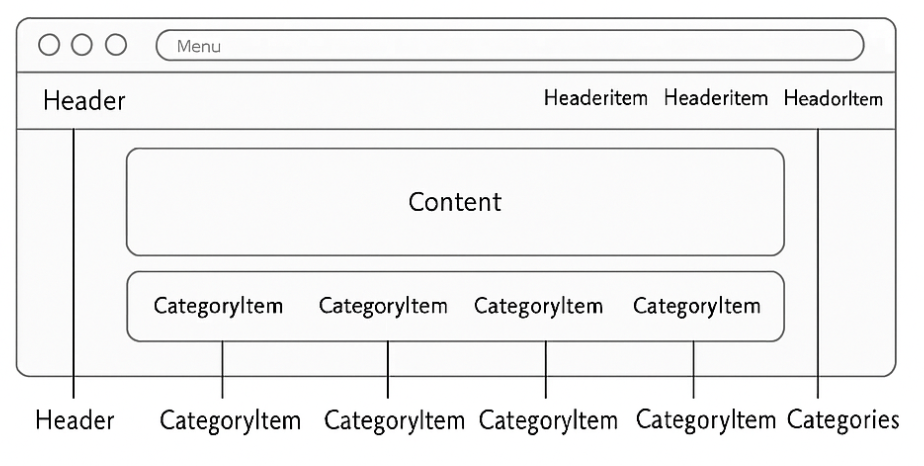
\includegraphics[width=0.85\textwidth]{REACT_NATIVE/images/A_text-based_digital_educational_graphic_offers_a_.png.png}
  \caption{Exemplo visual de componentização de um site com cabeçalho, categorias e conteúdo}
  \label{fig:componentizacao}
\end{figure}

Na Figura~\ref{fig:componentizacao}, temos uma interface simples de um site que foi dividida em componentes:

\begin{itemize}
  \item Um componente \texttt{Header}, responsável pela parte superior do site.
  \item Dentro do \texttt{Header}, componentes \texttt{HeaderItem} para cada item do menu.
  \item Um componente \texttt{Categorias}, que agrupa diversos componentes \texttt{CategoriaItem}.
  \item Outros elementos como a logo, barra de busca e sacola de compras também podem ser componentes reutilizáveis.
\end{itemize}

Essa flexibilidade é uma das maiores vantagens do React. Não existe uma única forma correta de dividir os componentes — essa decisão depende do projeto, da equipe e do contexto. O importante é que cada componente seja uma unidade funcional, reutilizável e de responsabilidade única.

\subsection*{Virtual DOM: performance com eficiência}

Outra inovação poderosa do React é o uso do \textit{Virtual DOM} — uma representação leve da estrutura de elementos da interface mantida em memória. Sempre que um componente sofre uma alteração (por exemplo, o usuário digita em um campo de texto), o React atualiza o Virtual DOM e compara com a versão anterior. Apenas as mudanças reais são aplicadas ao DOM do navegador.

Esse processo é conhecido como \textit{reconciliação} e é o que torna as aplicações React extremamente rápidas, pois evita recarregamentos desnecessários.

\subsection*{E o React Native?}

O React Native segue a mesma filosofia do React para web: dividir a interface em componentes reutilizáveis. A principal diferença está no ambiente de execução. Enquanto o React web manipula o DOM do navegador, o React Native se comunica com APIs nativas do sistema operacional por meio de uma ponte chamada \textit{Bridge}.

Essa ponte permite que o código JavaScript interaja diretamente com componentes nativos escritos em Java (Android) ou Swift/Objective-C (iOS). Com isso, conseguimos desenvolver aplicações verdadeiramente nativas, mas com a simplicidade e poder do React.



\section*{Código-fonte}
Código-fonte deste capítulo encontra-se em \href{https://github.com/hrausch/academico-react-native/tree/aula-04}{https://github.com/hrausch/academico-react-native/tree/aula-04} .


